
\chapter{Coverings}

\section{FIBERED PRODUCTS AND CARTESIAN SQUARES}

\subsection{Structure of a B-space}

Let B be a topological space.

DEFINITION 1. --- A topological B-space (or simply B-space) is a topological space X, equipped with a continuous map p from X to B. The map p is called the projection of the B-space X.

Let X, X' be B-spaces and p, \(p'\) their respective projections. A B-morphism from X to X' is a continuous map f from X to X' such that \(p' \circ f = p\) .

It is sometimes convenient to denote by \((X,p)\) the B-space obtained by equipping the topological space X with the continuous map p.

The composite of two B-morphisms is a B-morphism. The isomorphisms of B-spaces, also called B-isomorphisms, are the B-morphisms which are homeomorphisms.

Thus, if one calls the structure of B-space on a set X the data of a topology on X and a continuous map \(p: X \rightarrow B\) , one may take the B-morphisms as morphisms of the B-space structure (E, IV, p. 11).

Let X, \(X'\) be B-spaces. One denotes by \(\mathcal{C}_{\mathrm{B}}(\mathrm{X};\mathrm{X}')\) the set of B-morphisms from X to \(X'\) , \(\operatorname{Isom}_{\mathrm{B}}(\mathrm{X};\mathrm{X}')\) the set of B-isomorphisms from X to \(X'\) and \(\operatorname{Aut}_{\mathrm{B}}(\mathrm{X})\) the set of B-automorphisms of X, that is, the B-isomorphisms from X to X.

Let X be a B-space and p its projection. If one equips B with the structure of a B-space whose projection is \(Id_{B}\) , the set \(\mathcal{C}_{\mathrm{B}}(\mathrm{B};\mathrm{X})\) is the set of continuous sections (E, II, p. 18, def. 11) of p.

Let X be a B-space, p its projection, and b a point of B. The subspace \(\overline{p}^{1}(b)\) of X is called the fiber of X over b (or the fiber of p over b) and is denoted \(X_{b}\) . For a continuous map f from X to a B-space \(X'\) to be a B-morphism, it is necessary and sufficient that \(f(\mathrm{X}_{b})\) be contained in \(X_{b}'\) for all \(b \in B\) .

Let X be a B-space and p its projection. Let f be a continuous map from a topological space B' into B. A continuous map \(g: B' \to X\) such that \(p \circ g = f\) is called a continuous lift of f to X. In other words, if one endows B′ with the structure of a B-space with projection f, the continuous lifts of f to X are the B-morphisms from B′ to X.

\subsection{Operations on B-spaces}

Let B be a topological space.

Let X be a B-space and p its projection. Every topological subspace Y of X is endowed with the B-space structure whose projection is \(p \mid Y\) . Let A be a subspace of B; endowed with the map \(p_{\mathrm{A}}: \overline{p}^{1}(\mathrm{A}) \to \mathrm{A}\) induced by p by passing to subspaces, the topological space \(\overline{p}^{1}(\mathrm{A})\) is an A-space. It is called the A-space induced by \((\mathrm{X}, p)\) over A and is sometimes denoted \(X_{A}\) .

Let \((\mathrm{X}_{i})_{i\in\mathrm{I}}\) be a family of B-spaces, and let \(p_{i}\) be the projection of \(X_{i}\) . The sum space \(X = \coprod_{i\in I} X_{i}\) (TG, I, p. 15), equipped with the map \(p: X \to B\) defined by \(p(i,x) = p_{i}(x)\) (for \(i \in I\) and \(x \in X_{i}\) ), is a B-space called the sum of the family of B-spaces \((\mathrm{X}_{i})_{i\in\mathrm{I}}\) . The canonical injections \(X_{i} \to X\) are B-morphisms.

Let X be a B-space, p its projection, and let R be an equivalence relation on X. Denote by X/R the quotient space (TG, I, p. 20, def. 3). If the map \(p: X \rightarrow B\) is compatible with the relation R (E, II, p. 44), the map \(p'\colon X/R \to B\) induced by p by passing to the quotient is continuous (TG, I, p. 21, prop. 6); the B-space obtained by endowing X/R with the projection \(p'\) is then called the quotient B-space of X by the relation R.

\subsection{Fibered product of two B-spaces}

Let B be a topological space, and let X and X′ be B-spaces, with p and p′ their respective projections. Denote by X ×B X′ the topological subspace of X × X′ consisting of the pairs \((x, x')\) such that \(p(x) = p'(x')\) . The map \(q: X \times_{B} X' \to B\) defined by \(q(x, x') = p(x)\) is continuous.

DEFINITION 2. --- The topological space X × \(_{B}\) X' is called the fiber product of X and X' over B. The B-space obtained by endowing X × \(_{B}\) X' with the map q is called the product B-space of X and X'.

The restrictions to \(X \times_{B} X'\) of the projections of \(X \times X'\) onto X and X' are still denoted \(pr_{1}\) and \(pr_{2}\) and are called the first and second projections of the fibered product. They are continuous and are B-morphisms, since we have \(q = p \circ pr_{1} = p' \circ pr_{2}\) .

Note that \(X \times_{B} X'\) may be empty even if X and \(X'\) are nonempty: indeed, the relation \(X \times_{B} X' = \varnothing\) is equivalent to saying that \(p(X)\) and \(p'(X')\) are disjoint.

Let Y be a B-space and let \(u\colon\mathrm{Y}\to\mathrm{X}, u'\colon\mathrm{Y}\to\mathrm{X}'\) be B-morphisms. There exists a unique B-morphism \(v\colon\mathrm{Y}\to\mathrm{X}\times_{\mathrm{B}}\mathrm{X}'\) such that \(\mathrm{pr}_{1}\circ v=u\) and \(\mathrm{pr}_{2}\circ v=u'\) (universal property of the product B-space of two B-spaces): it is the map \(y\mapsto(u(y),u'(y))\) from Y into \(\mathrm{X}\times_{\mathrm{B}}\mathrm{X}'\) , which is sometimes denoted \((u,u')\) .

Let X, X', Y, Y' be B-spaces, and let \(f: X \to Y\) , \(f': X' \to Y'\) be B-morphisms. The map \((x, x') \mapsto (f(x), f'(x'))\) is a B-morphism from \(X \times_{B} X'\) into \(Y \times_{B} Y'\) , denoted \(f \times_{B} f'\) and called the extension of f and \(f'\) to fibered products.

Examples. --- 1) Let X and X' be B-spaces; then the map \((x, x') \mapsto (x', x)\) defines a B-isomorphism of \(X \times_{B} X'\) onto \(X' \times_{B} X\) .

\begin{enumerate}
\def\labelenumi{\arabic{enumi})}
\setcounter{enumi}{1}
\item
  Let X, \(X'\) , \(X''\) be B-spaces and p, \(p'\) , \(p''\) their respective projections. The product B-space \((\mathrm{X} \times_{\mathrm{B}} \mathrm{X}') \times_{\mathrm{B}} \mathrm{X}''\) is the topological subspace \(X \times_{B} X' \times_{B} X''\) of \(X \times X' \times X''\) consisting of triples \((x, x', x'')\) such that \(p(x) = p'(x') = p''(x''), \text{ equipped with the projection } q: X \times_{B} X' \times_{B} X'' \to B\) defined by \(q(x, x', x'') = p(x)\) .
\item
  Let X be a B-space and p its projection. The fibered product \(X \times_{B} X\) of X and X over B is called the fibered square of X. It is the subspace of \(X \times X\) consisting of the pairs \((x, x')\) such that \(p(x) = p(x')\) . It is equipped with the structure of a B-space whose projection is the map \((x, x') \mapsto p(x)\) . The diagonal \(\Delta_{X}\) of \(X \times X\) (E, II, p. 13) is contained in \(X \times_{B} X\) ; it is also called the diagonal of \(X \times_{B} X\) . The map \(x \mapsto (x, x)\) from X to \(X \times_{B} X\) is a B-morphism, called the diagonal B-morphism and often denoted \(\delta_{X}\) ; it defines a B-isomorphism from X onto \(\Delta_{X}\) (TG, I, p. 25, cor. 2).
\item
  Let \((\mathrm{B}_{i})_{i\in\mathrm{I}}\) be a family of topological spaces and, for every \(i\in I\) , let \((\mathrm{X}_{i},p_{i})\) and \((\mathrm{Y}_{i},q_{i})\) be \(B_{i}\)-spaces. Set \(B=\prod_{i\in I}B_{i}\) , \(X=\prod_{i\in I}X_{i}\) and \(Y=\prod_{i\in I}Y_{i}\) . Equipped with the continuous map \(p=\prod_{i}p_{i}\) (resp. \(q=\prod_{i}q_{i}\) ), the topological space X (resp. Y) is a B-space. By the associativity isomorphism for topological products from \(\prod_{i}(\mathrm{X}_{i}\times\mathrm{Y}_{i})\) onto \((\prod_{i}\mathrm{X}_{i})\times(\prod_{i}\mathrm{Y}_{i})=\mathrm{X}\times\mathrm{Y}\) (TG, I, p. 25, prop. 2), the subspace \(\prod_{i}(\mathrm{X}_{i}\times_{\mathrm{B}_{i}}\mathrm{Y}_{i})\) of \(\prod_{i}(\mathrm{X}_{i}\times\mathrm{Y}_{i})\) is identified with \(X\times_{B}Y\) .
\item
  Let \((\mathrm{X}_{i})_{i\in\mathrm{I}}\) and \((\mathrm{Y}_{j})_{j\in\mathrm{J}}\) be families of B-spaces. Let X and Y be their sums. For every \((i,j)\in\mathrm{I}\times\mathrm{J}\) , the map \((x,y)\mapsto((i,x),(j,y))\) is a B-isomorphism from \(X_{i}\times_{B}Y_{j}\) onto the subspace \((\{i\}\times\mathrm{X}_{i})\times_{\mathrm{B}}(\{j\}\times\mathrm{Y}_{j})\) of \(X\times_{B}Y\) . Since the latter form a partition of \(X\times_{B}Y\) into open subsets, the map
\end{enumerate}

\[
h \colon \coprod_ {(i, j) \in \mathrm{I} \times \mathrm{J}} (\mathrm{X} _ {i} \times_ {\mathrm{B}} \mathrm{Y} _ {j}) \to \mathrm{X} \times_ {\mathrm{B}} \mathrm{Y}
\]

defined by \(h((i,j),(x,y)) = ((i,x),(j,y))\) is a B-isomorphism.

\subsection{Change of basis}

Let B, B' be topological spaces and \(f\colon\mathrm{B}^{\prime}\to\mathrm{B}\) a continuous map. Let X be a B-space. The map \(f\) endows B' with a B-space structure, which allows one to define the fibered product \(\mathrm{B}^{\prime}\times_{\mathrm{B}}\mathrm{X}\) . This, equipped with the map \(\mathrm{pr}_{1}\colon\mathrm{B}^{\prime}\times_{\mathrm{B}}\mathrm{X}\to\mathrm{B}^{\prime}\) , is a B'-space called the B'-space induced from the B-space X by the base change \(f\colon\mathrm{B}^{\prime}\to\mathrm{B}\) (or by the base change from B to B' along f). It is also called the inverse-image B'-space of X under f. It is denoted \(f^{*}(\mathrm{X})\) , or sometimes \(X_{B'}\) when there is no possible confusion about the map f.

When B' is a subspace of B and \(f: B' \to B\) is the canonical injection, the map \((b', x) \mapsto x\) from \(B' \times_{B} X\) onto \(p^{-1}(B')\) (where p is the projection of X) is a B'-isomorphism from \(f^{*}(X)\) onto the B'-space induced by X over B'.

Let Y be a second B-space and \(u\colon X\to Y\) a B-morphism. The map \(\mathrm{Id}_{\mathrm{B}^{\prime}}\times_{\mathrm{B}}u\colon \mathrm{B}^{\prime}\times_{\mathrm{B}}\mathrm{X}\to \mathrm{B}^{\prime}\times_{\mathrm{B}}\mathrm{Y}\) is a \(\mathrm{B}'\) -morphism, called the \(\mathrm{B}'\) -morphism induced from the B-morphism \(u\) by the base change \(f\colon \mathrm{B}'\to \mathrm{B}\) and sometimes denoted \(f^{*}(u)\) , or \(u_{\mathrm{B}'}\) when there is no possible confusion about the map \(f\) . It is the unique \(\mathrm{B}'\) -morphism \(v\) from \(\mathrm{B}'\times_{\mathrm{B}}\mathrm{X}\) into \(\mathrm{B}'\times_{\mathrm{B}}\mathrm{Y}\) such that \(\mathrm{pr}_2\circ v = u\circ \mathrm{pr}_2\) .

Let B'' be a topological space and let \(g: B'' \to B'\) be a continuous map. Then the map given by \((b'', (b', x)) \mapsto (b'', x)\) is a canonical isomorphism of B''-spaces from \(g^{*}(f^{*}(\mathrm{X}))\) onto \((f \circ g)^{*}(\mathrm{X})\) .

\subsection{Fibered product of a family of B-spaces}

Let \((\mathrm{X}_{i})_{i\in\mathrm{I}}\) be a family of B-spaces. Let \(p_{i}\colon X_{i}\to B\) be their projections. Denote by \(\prod_{B}X_{i}\) the topological subspace of \(B\times\prod_{i\in I}X_{i}\) consisting of the pairs \((b,(x_{i})_{i\in\mathrm{I}})\) such that \(p_{i}(x_{i})=b\) for all \(i\in I\) . The map \(p\colon\prod_{B}X_{i}\to B\) defined by \(p(b,(x_{i})_{i\in\mathrm{I}})=b\) is continuous.

DEFINITION 3. --- The topological space \(\prod_{\mathrm{B}} \mathrm{X}_i\) is called the fibered product of the family \((\mathrm{X}_i)_{i \in \mathrm{I}}\) over B. The B-space obtained by endowing \(\prod_{\mathrm{B}} \mathrm{X}_i\) with the map p is called the product B-space of the family \((\mathrm{X}_i)_{i \in \mathrm{I}}\) .

Let \(j \in I\) . The map \((b, x) \mapsto \operatorname{pr}_j(x)\) from \(\prod_B X_i\) into \(X_j\) is called the projection of index \(j\) of the fibered product and is still denoted \(\operatorname{pr}_j\) . It is continuous. It is a B-morphism, since one has \(p = p_j \circ \operatorname{pr}_j\) .

Let Y be a B-space and q its projection. For every \(i \in I\) , let \(u_i \colon Y \to X_i\) be a B-morphism. There exists a unique B-morphism \(v \colon Y \to \prod_{B} X_i\) such that \(pr_i \circ v = u_i\) for all \(i \in I\) (universal property of the product B-space): it is the map from Y into \(\prod_{B} X_i\) , defined by \(y \mapsto (q(y), (u_i(y))_{i \in I})\) , which is sometimes denoted \((u_i)_{i \in I}\) .

Let \((\mathrm{X}_{i})_{i\in\mathrm{I}}\) and \((\mathrm{Y}_{i})_{i\in\mathrm{I}}\) be families of B-spaces and, for every \(i\in I\) , let \(f_{i}\colon X_{i}\to Y_{i}\) be a B-morphism. The map \((b,(x_{i})_{i\in\mathrm{I}})\mapsto(b,(f_{i}(x_{i}))_{i\in\mathrm{I}})\) is a B-morphism from \(\prod_{B}X_{i}\) into \(\prod_{B}Y_{i}\) , denoted \(\prod_{B}f_{i}\) and called the extension of the family \((f_{i})_{i\in\mathrm{I}}\) to fibered products.

Examples. --- 1) When the set I is empty, the set \(\prod_{i\in I}X_i\) is reduced to a single element and the B-space \(\prod_{B}X_{i}\) is identified with B (endowed with the projection \(Id_B\) ).

\begin{enumerate}
\def\labelenumi{\arabic{enumi})}
\setcounter{enumi}{1}
\item
  When I is nonempty, the map \((b,x)\mapsto x\) from \(B\times\prod_{i\in I}X_{i}\) into \(\prod_{i\in I}X_{i}\) induces, by passage to subspaces, a homeomorphism from \(\prod_{B}X_{i}\) onto the subspace of \(\prod_{i\in I}X_{i}\) consisting of families \((x_{i})_{i\in I}\) such that \(p_{i}(x_{i})=p_{j}(x_{j})\) for all \(i,j\in I\) . This subspace will be called, by abuse of language, the fibered product of the family \((\mathrm{X}_{i})_{i\in\mathrm{I}}\) .
\item
  When the set I has one element \(\alpha\) (resp. two elements \(\alpha\) and \(\beta\) ; resp. three elements \(\alpha\) , \(\beta\) , \(\gamma\) ), the map \(\mathrm{pr}_{\alpha}\) (resp. \((\mathrm{pr}_{\alpha}, \mathrm{pr}_{\beta})\) ; resp. \((\mathrm{pr}_{\alpha}, \mathrm{pr}_{\beta}, \mathrm{pr}_{\gamma})\) ) from \(\prod_{\mathrm{B}} \mathrm{X}_i\) into \(\mathrm{X}_{\alpha}\) (respectively, into \(\mathrm{X}_{\alpha} \times_{\mathrm{B}} \mathrm{X}_{\beta}\) ; respectively, into \(\mathrm{X}_{\alpha} \times_{\mathrm{B}} \mathrm{X}_{\beta} \times_{\mathrm{B}} \mathrm{X}_{\gamma}\) ) is a B-isomorphism. This will allow us to deduce the properties of the fibered product of two or three B-spaces from those of the fibered product of families of B-spaces.
\end{enumerate}

Let \((\mathrm{X}_{i})_{i\in\mathrm{I}}\) be a family of B-spaces and let J be a subset of I. From the map \(Id_{B}\times pr_{J}\) from \(B\times\prod_{i\in I}X_{i}\) into \(B\times\prod_{i\in J}X_{i}\) , by passage to subsets, one obtains a B-morphism \(\prod_{i\in I}X_{i}\to\prod_{i\in J}X_{i}\) . We still denote it by \(pr_{J}\) and call it the projection with index J of the fibered product.

Let \((\mathrm{X}_{i})_{i\in\mathrm{I}}\) be a family of B-spaces. Let \((\mathrm{J}_{\lambda})_{\lambda\in\mathrm{L}}\) be a partition of I. The map \((\mathrm{pr}_{\mathrm{J}_{\lambda}})_{\lambda\in\mathrm{L}}\) from \(\prod_{i\in I}X_{i}\to\prod_{\lambda\in L}\left(\prod_{i\in J_{\lambda}}X_{i}\right)\) is a B-isomorphism ("associativity" of fibered products of B-spaces).

\subsection{Cartesian squares}

Let B, B′, X, X′ be topological spaces and let \(f: B' \to B\) , \(f': X' \to X\) , \(p: X \to B\) , \(p': X' \to B'\) be continuous maps. One can represent such a quadruple \((f, f', p, p')\) by a diagram

\begin{enumerate}
\def\labelenumi{(\arabic{enumi})}
\tightlist
\item
\end{enumerate}

\pandocbounded{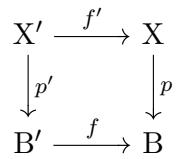
\includegraphics[keepaspectratio]{images/part001_dd3067cf.jpg}}

(E, II, p. 14). We shall then say, “Consider the square diagram (1),” or simply “the square (1),” instead of saying, “Consider the quadruple \(f,f^{\prime},p,p^{\prime}\) of continuous maps.” The square (1) is said to be commutative if the equality

\[
f \circ p ^ {\prime} = p \circ f ^ {\prime}
\]

is satisfied. In this case, one often endows B′, X, and X′ with the structures of B-spaces defined by the maps f, p, and \(f \circ p' = p \circ f'\) respectively; the maps \(p'\) and \(f'\) are then B-morphisms.

DEFINITION 4. --- We say that the square (1) is a Cartesian square of topological spaces (or, simply, that it is Cartesian) if it is commutative and if, for every topological space Y and every pair of continuous maps u: Y → B', v: Y → X such that f ∘ u = p ∘ v, there exists a unique continuous map w: Y → X' such that p' ∘ w = u and f' ∘ w = v.

For the square (1) to be Cartesian, it is necessary and sufficient that the square

(1')

\pandocbounded{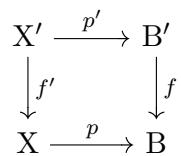
\includegraphics[keepaspectratio]{images/part001_f0fdde30.jpg}}

is Cartesian.

PROPOSITION 1. --- For the square (1) to be Cartesian, it is necessary and sufficient that it be commutative and that, for every B-space Y and every pair of B-morphisms \(u\colon Y \to B'\) , \(v\colon Y \to X\) there exists a unique B-morphism \(w\colon Y \to X'\) such that \(p' \circ w = u\) and \(f' \circ w = v\) .

Suppose that the square (1) is Cartesian. Let Y be a B-space and let \(u: Y \to B'\) and \(v: Y \to X\) be B-morphisms. The maps \(f \circ u\) and \(p \circ v\) are both equal to the projection of the B-space Y; the unique continuous map w such that \(p' \circ w = u\) and \(f' \circ w = v\) is then a B-morphism. This proves the necessity of the condition.

Conversely, suppose this condition is satisfied. Let Y be a topological space and let \(u \colon \mathrm{Y} \to \mathrm{B}'\) and \(v \colon \mathrm{Y} \to \mathrm{X}\) be continuous maps such that \(f \circ u = p \circ v\) . When Y is endowed with the B-space structure defined by \(f \circ u\) , \(u\) and \(v\) are B-morphisms. Every continuous map \(w \colon \mathrm{Y} \to \mathrm{X}'\) such that \(p' \circ w = u\) and \(f' \circ w = v\) is a B-morphism, so there exists exactly one such map.

PROPOSITION 2. --- Let B, B' and X be topological spaces and p: X → B, f: B' → B continuous maps.

\begin{enumerate}
\def\labelenumi{\alph{enumi})}
\tightlist
\item
  The square
\end{enumerate}

\[
\begin{array}{c} \mathrm{B} ^ {\prime} \times_ {\mathrm{B}} \mathrm{X} \xrightarrow {\mathrm{pr} _ {2}} \mathrm{X} \\ \Biggl \downarrow \mathrm{pr} _ {1} \\ \mathrm{B} ^ {\prime} \xrightarrow {f} \mathrm{B} \end{array}\tag{2}
\]

is a Cartesian square.

\begin{enumerate}
\def\labelenumi{\alph{enumi})}
\setcounter{enumi}{1}
\tightlist
\item
  For every commutative square
\end{enumerate}

\[
\begin{array}{c} \mathrm {X^ {\prime}} \xrightarrow {f ^ {\prime}} \mathrm{X} \\ \Big \downarrow_ {p ^ {\prime}} \\ \mathrm {B^ {\prime}} \xrightarrow {f} \mathrm{B} \end{array}\tag{3}
\]

there exists a unique continuous map \(h: X' \to B' \times_{B} X\) such that \(pr_{1} \circ h = p'\) and \(pr_{2} \circ h = f'\) .

\begin{enumerate}
\def\labelenumi{\alph{enumi})}
\setcounter{enumi}{2}
\tightlist
\item
  The commutative square (3) is Cartesian if and only if h is a homeomorphism.
\end{enumerate}

Assertion \(a\) ) follows from Proposition 1 and the universal property of the product of two B-spaces in the category of B-spaces (I, p. 3). Assertion \(b\) ) follows from it.

If the square (3) is Cartesian, there exists a unique continuous map \(h'\colon B'\times_{B}X\to X'\) such that \(f'\circ h' = pr_{2}\) and \(p'\circ h' = pr_{1}\) . We have \(f'\circ h'\circ h = f'\) and \(p'\circ h'\circ h = p'\) , whence \(h'\circ h = Id_{X'}\) since the square (3) is Cartesian. We have \(pr_{1}\circ h\circ h' = pr_{1}\) and \(pr_{2}\circ h\circ h' = pr_{2}\) , whence \(h\circ h' = Id_{B'\times_{B}X}\) since the square (2) is Cartesian. This proves that h is a homeomorphism.

Conversely, suppose that h is a homeomorphism; since square (2) is Cartesian, square (3) is also Cartesian.

The map \(h \colon \mathrm{X}' \to \mathrm{B}' \times_{\mathrm{B}} \mathrm{X}\) whose existence and uniqueness is asserted by part \(b)\) of the preceding proposition will be called canonical: it is the map denoted \((p', f')\) in I, p. 3.

PROPOSITION 3. --- Let

\[
\begin{array}{c} \mathrm {X^ {\prime}} \xrightarrow {f ^ {\prime}} \mathrm{X} \\ \Big \downarrow_ {p ^ {\prime}} \\ \mathrm {B^ {\prime}} \xrightarrow {f} \mathrm{B} \end{array}
\]

a Cartesian square. For any continuous section s of \(p'\) , the map \(f'\circ s\) is a continuous lift of f to X. The map \(s\mapsto f'\circ s\) is a bijection from \(\mathcal{C}_{\mathrm{B}'}(\mathrm{B}';\mathrm{X}')\) onto \(\mathcal{C}_{\mathrm{B}}(\mathrm{B}';\mathrm{X})\) .

If \(s \colon B' \to X'\) is a continuous section of \(p'\) , we have \(p \circ f' \circ s = f \circ p' \circ s = f\) , which proves that \(f' \circ s\) is a continuous lifting of \(f\) to X, i.e., a B-morphism from \(B'\) into X. Conversely, let \(g \colon B' \to X\) be a B-morphism. We have \(f \circ \mathrm{Id}_{\mathrm{B}'} = p \circ g\) ; there therefore exists, by definition of a Cartesian square, a unique continuous map \(s \colon B' \to X'\) such that \(p' \circ s = \mathrm{Id}_{\mathrm{B}'}\) and \(f' \circ s = g\) , whence the proposition.

\subsection{Cartesian squares constructed by passing to subspaces}

PROPOSITION 4. --- Let

\[
\begin{array}{c} \mathrm {X^ {\prime}} \xrightarrow {f ^ {\prime}} \mathrm{X} \\ \Big \downarrow_ {p ^ {\prime}} \\ \mathrm {B^ {\prime}} \xrightarrow {f} \mathrm{B} \end{array}\tag{4}
\]

a Cartesian square and let \(B_{0}\) , \(B_{0}^{\prime}\) , \(X_{0}\) be subspaces of B, \(B^{\prime}\) and X, respectively. Suppose we have \(f(B_{0}^{\prime}) \subset B_{0}\) , \(p(X_{0}) \subset B_{0}\) and let us set \(X_{0}^{\prime} = \overline{p'}^{1}(B_{0}^{\prime}) \cap \overline{f'}^{1}(X_{0})\) . Then, the square

\[
\begin{array}{c} \mathrm{X} _ {0} ^ {\prime} \xrightarrow {f _ {0} ^ {\prime}} \mathrm{X} _ {0} \\ \Biggl \downarrow p _ {0} ^ {\prime} \\ \mathrm{B} _ {0} ^ {\prime} \xrightarrow {f _ {0}} \mathrm{B} _ {0} \end{array}\tag{4'}
\]

(where the maps \(f_0\) , \(f_0'\) , \(p_0\) , \(p_0'\) are deduced from \(f\) , \(f'\) , \(p\) , \(p'\) respectively by passing to subsets) is Cartesian.

Consider the canonical map \(h \colon X' \to B' \times_B X\) deduced from the commutative diagram (4). Since square (4) is Cartesian, \(h\) is a homeomorphism. By construction, we have \(X_0' = h^{-1}(B_0' \times_{B_0} X_0)\) and the mapping \(h_0 \colon X_0' \to B_0' \times_{B_0} X_0\) deduced from the commutative diagram ( \(4'\) ) is deduced from \(h\) by passing to subsets. It is therefore a homeomorphism, and the square ( \(4'\) ) is Cartesian (prop. 2).

COROLLARY. --- Let

\pandocbounded{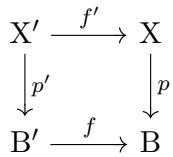
\includegraphics[keepaspectratio]{images/part001_2907af81.jpg}}

a Cartesian square.

\begin{enumerate}
\def\labelenumi{\alph{enumi})}
\item
  For every point \(b'\) of \(B'\) , the map \(f'\) induces a homeomorphism of the fiber \(X_{b'}'\) of \(p'\) onto the fiber \(X_{f(b')}\) of \(p\) .
\item
  If the map p is injective (resp. surjective, resp. bijective), then so is \(p'\) .
\end{enumerate}

Let \(b'\) be a point of B'. Set \(b = f(b')\) . For all \(x' \in X_{b'}'\) , we have \(p(f'(x')) = f(p'(x')) = f(b') = b\) , whence \(f'(x') \in X_b\) . This proves that one has \(X_{b'}' \subset \overline{f'}^{1}(X_b)\) . In Proposition 4, take \(B_0 = \{b\}\) , \(B_0' = \{b'\}\) and \(X_0 = X_b\) ; we then have \(X_0' = X_{b'}'\) , whence the assertion \(a\) ).

For the map p to be injective (resp. surjective, resp. bijective), it is necessary and sufficient that the cardinality of each of its fibers be at most (resp. at least, resp. equal to) 1. Assertion b) follows from this.

Example. --- Let \((X,p)\) be a B-space and A a subspace of B. The square

\[
\begin{array}{c} \overline {{p}} ^ {1} (\mathrm{A}) \xrightarrow {j} \mathrm{X} \\ \Biggl \downarrow p _ {\mathrm{A}} \\ \mathrm{A} \xrightarrow {i} \mathrm{B} \end{array}\tag{5}
\]

(where i and j are the canonical injections) is cartesian.

In particular, if A and A' are subspaces of the topological space B, the square

\begin{enumerate}
\def\labelenumi{(\arabic{enumi})}
\setcounter{enumi}{5}
\tightlist
\item
\end{enumerate}

\pandocbounded{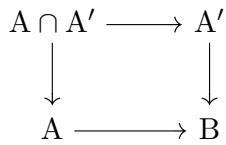
\includegraphics[keepaspectratio]{images/part001_a4278a10.jpg}}

(where the arrows are the canonical injections) is cartesian.

\subsection{Cartesian squares constructed by products, fibered products, and sums}

PROPOSITION 5. --- Let I be a set and, for every \(i \in I\) , let

\[
\begin{array}{c} \mathrm{X} _ {i} ^ {\prime} \xrightarrow {f _ {i} ^ {\prime}} \mathrm{X} _ {i} \\ \Big \downarrow p _ {i} ^ {\prime} \\ \mathrm{B} _ {i} ^ {\prime} \xrightarrow {f _ {i}} \mathrm{B} _ {i} \end{array}\tag{7}
\]

a cartesian square. The square

\[
\begin{array}{c} \prod_ {i \in \mathrm{I}} \mathrm{X} _ {i} ^ {\prime} \xrightarrow {f ^ {\prime}} \prod_ {i \in \mathrm{I}} \mathrm{X} _ {i} \\ \Biggl \downarrow^ {p ^ {\prime}} \qquad \qquad \qquad \qquad \Biggl \downarrow^ {p} \\ \prod_ {i \in \mathrm{I}} \mathrm{B} _ {i} ^ {\prime} \xrightarrow {f} \prod_ {i \in \mathrm{I}} \mathrm{B} _ {i} \end{array}\tag{ (7') }
\]

\((\text{where } f, f', p, p' \text{ are the extensions of the families } (f_i), (f'_i), (p_i), (p'_i) \text{ to products}) \text{ is Cartesian.}\)

Let Y be a topological space, and let \(u \colon \mathrm{Y} \to \prod_{i} \mathrm{B}_{i}'\) and \(v \colon \mathrm{Y} \to \prod_{i} \mathrm{X}_{i}\) be continuous maps such that \(f \circ u = p \circ v\) . For \(i \in \mathrm{I}\) , set \(u_{i} = \mathrm{pr}_{i} \circ u\) and \(v_{i} = \mathrm{pr}_{i} \circ v\) ; we have \(f_{i} \circ u_{i} = p_{i} \circ v_{i}\) and there exists a unique continuous map \(w_{i} \colon \mathrm{Y} \to \mathrm{X}_{i}'\) such that \(p_{i}' \circ w_{i} = u_{i}\) and \(f_{i}' \circ w_{i} = v_{i}\) . Then, the map \(w = (w_{i})\) is a continuous map from Y into \(\prod_{i} \mathrm{X}_{i}'\) such that \(p' \circ w = u\) and \(f' \circ w = v\) and it is the only one having these properties.

COROLLARY 1. --- Let X be a B-space, let p be its projection, and let F be a topological space. The square

\[
\begin{array}{c} \mathrm{X} \times \mathrm{F} \xrightarrow {\operatorname{pr} _ {1}} \mathrm{X} \\ \Biggl \downarrow p \times \mathrm{Id} _ {\mathrm{F}} \\ \mathrm{B} \times \mathrm{F} \xrightarrow {\operatorname{pr} _ {1}} \mathrm{B} \end{array}\tag{8}
\]

is Cartesian.

Let P be a topological space reduced to a point. Corollary 1 follows from Prop. 5 applied to the Cartesian squares

\[
\begin{array}{l} \mathrm{X} \xrightarrow {\mathrm{Id} _ {\mathrm{X}}} \mathrm{X} \\ \Big \downarrow_ {p} \qquad \Big \downarrow_ {p} \\ \mathrm{B} \xrightarrow {\mathrm{Id} _ {\mathrm{B}}} \mathrm{B} \end{array} \qquad \text {and} \qquad \begin{array}{l} \mathrm{F} \longrightarrow \mathrm{P} \\ \Big \downarrow_ {\mathrm{Id} _ {\mathrm{F}}} \qquad \Big \downarrow_ {\mathrm{Id} _ {\mathrm{P}}} \\ \mathrm{F} \longrightarrow \mathrm{P}. \end{array}
\]

Let B and B' be topological spaces, and let \(f: B' \to B\) be a continuous map. Let I be a set and, for every \(i \in I\) , let \(X_i\) be a B-space, \(X'_i\) be a B'-space, and \(f'_i: X'_i \to X_i\) be a continuous map such that the square

\[
\begin{array}{c} \mathrm{X} _ {i} ^ {\prime} \xrightarrow {f _ {i} ^ {\prime}} \mathrm{X} _ {i} \\ \Big \downarrow \\ \mathrm{B} ^ {\prime} \xrightarrow {f} \mathrm{B} \end{array}\tag{9}
\]

is commutative. There exists a unique continuous map

\[
f ^ {\prime} \colon \prod_ {i \in \mathrm{I}} \mathrm{X} _ {i} ^ {\prime} \to \prod_ {i \in \mathrm{I}} \mathrm{X} _ {i}
\]

such that \(pr_{i} \circ f' = f_{i}' \circ pr_{i}\) for all \(i \in I\) and such that the square

\[
\begin{array}{c} \prod_ {i \in I} X _ {i} ^ {\prime} \xrightarrow {f ^ {\prime}} \prod_ {i \in I} X _ {i} \\ \Big \downarrow \qquad \qquad \qquad \qquad \Big \downarrow \\ B ^ {\prime} \xrightarrow {f} B \end{array}\tag{ (9') }
\]

is commutative (this last condition following from the others if I ≠ ∅): it is the map deduced from the map

\[
f \times \prod_ {i \in \mathrm{I}} f _ {i} ^ {\prime} \colon \mathrm{B} ^ {\prime} \times \prod_ {i \in \mathrm{I}} \mathrm{X} _ {i} ^ {\prime} \to \mathrm{B} \times \prod_ {i \in \mathrm{I}} \mathrm{X} _ {i}
\]

by passing to subsets. With these notations:

COROLLARY 2. --- If the square (9) is Cartesian for every \(i \in I\) , then the square ( \(9'\) ) is Cartesian.

From prop. 5 one deduces a Cartesian square

\[
\begin{array}{c} \mathrm{B} ^ {\prime} \times \prod_ {i} \mathrm{X} _ {i} ^ {\prime} \xrightarrow {\operatorname{Id} _ {\mathrm{B}} \times \prod_ {i} f _ {i} ^ {\prime}} \mathrm{B} \times \prod_ {i} \mathrm{X} _ {i} \\ \Biggl \downarrow \\ \mathrm{B} ^ {\prime} \times (\mathrm{B} ^ {\prime}) ^ {\mathrm{I}} \xrightarrow {f \times \prod_ {i} f} \mathrm{B} \times \mathrm{B} ^ {\mathrm{I}}  . \end{array}
\]

Denote by \(\Delta_{\mathrm{B}^{\prime}}\) and \(\Delta_{\mathrm{B}}\) the diagonals of \(\mathrm{B}^{\prime}\times (\mathrm{B}^{\prime})^{\mathrm{I}}\) and \(\mathrm{B}\times \mathrm{B}^{\mathrm{I}}\) . The diagram

\[
\begin{array}{c} \prod_ {i \in \mathrm{I}} X _ {i} ^ {\prime} \xrightarrow {f ^ {\prime}} \prod_ {i \in \mathrm{I}} X _ {i} \\ \Big \downarrow \qquad \qquad \qquad \Big \downarrow \\ \Delta_ {\mathrm{B} ^ {\prime}} \xrightarrow {} \Delta_ {\mathrm{B}} \end{array}
\]

deduced from the preceding one by passing to subspaces is Cartesian (I, p. 9, prop. 4). It is identified with diagram (9').

Example 1. --- Let

\[
\begin{array}{c} \mathrm {X^ {\prime}} \xrightarrow {f ^ {\prime}} \mathrm{X} \\ \Big \downarrow_ {p ^ {\prime}} \\ \mathrm {B^ {\prime}} \xrightarrow {f} \mathrm{B} \end{array}
\]

a Cartesian square. Then Corollary 2 provides a Cartesian square

\[
\begin{array}{c} \mathrm {X^ {\prime} \times_ {B^ {\prime}} X^ {\prime}} \xrightarrow {\varphi} \mathrm {X\times_ {B} X} \\ \Big \downarrow \\ \mathrm {B^ {\prime} \xrightarrow {f} B}. \end{array}
\]

We have the relation \(\overline{\varphi}^{1}(\Delta_{\mathrm{X}}) = \Delta_{\mathrm{X}^{\prime}}\) . Indeed, by Proposition 2 of I, p. 8, it suffices to consider the case where \(\mathrm{X}' = \mathrm{B}' \times_{\mathrm{B}} \mathrm{X}\) . Let then \(((b,x),(b,x'))\) be an element of \(X^{\prime} \times_{B^{\prime}} X^{\prime}\) with \(b \in B^{\prime}\) and \(x, x^{\prime} \in X\) . This element belongs to \(\overline{\varphi}^{1}(\Delta_{\mathrm{X}})\) if and only if \(x = x^{\prime}\) .

PROPOSITION 6. --- Let I be a set and, for every \(i \in I\) , let

\[
\begin{array}{c} \mathrm{X} _ {i} ^ {\prime} \xrightarrow {f _ {i} ^ {\prime}} \mathrm{X} \\ \Biggl \downarrow p _ {i} ^ {\prime} \\ \mathrm{B} _ {i} ^ {\prime} \xrightarrow {f _ {i}} \mathrm{B} \end{array}\tag{10}
\]

a Cartesian square. Let X' and B' be the sum spaces of the families \((X'_i)\) and \((B'_i)\), respectively. Let f: B' → B, f': X' → X, and p': X' → B' be the maps induced from the families \((f_i)\), \((f'_i)\), and \((p'_i)\), respectively. The square

\((10')\)

\pandocbounded{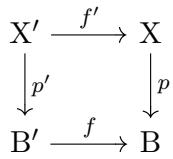
\includegraphics[keepaspectratio]{images/part001_48571453.jpg}}

is Cartesian.

The maps \(f\) , \(f'\) , and \(p'\) are continuous. The commutativity of the square \((10')\) follows from its definition. Let \(h_i\) denote the canonical homeomorphism from \(\mathrm{X}_i'\) onto \(\mathrm{B}_i' \times_{\mathrm{B}} \mathrm{X}\) (I, p. 8, Proposition 2) and let \(h: \mathrm{X}' \to \mathrm{B}' \times_{\mathrm{B}} \mathrm{X}\) be the canonical map (loc. cit.). We have \(h = h'' \circ h'\) , where \(h': \mathrm{X}' \to \coprod (\mathrm{B}_i' \times_{\mathrm{B}} \mathrm{X})\) is the homeomorphism induced by the \(h_i\) and \(h'': \coprod (\mathrm{B}_i' \times_{\mathrm{B}} \mathrm{X}) \to (\coprod \mathrm{B}_i') \times_{\mathrm{B}} \mathrm{X}\) is the one defined in Example 5 of I, p. 4. We conclude by Proposition 2 of I, p. 8.

Example 2. --- Let \((X,p)\) be a B-space and let \((\mathrm{A}_{k})_{k\in\mathrm{K}}\) be a family of subspaces of B. Let A be the sum space of the family \((\mathrm{A}_{k})_{k\in\mathrm{K}}\) and let Y be the sum space of the family \((\overline{p}^{1}(\mathrm{A}_{k}))_{k\in\mathrm{K}}\) ; let us denote by \(i: A \to B\) , \(j: Y \to X\) , and \(p': Y \to A\) the maps induced by the canonical injections of \(A_{k}\) into B, the canonical injections of \(\overline{p}^{1}(\mathrm{A}_{k})\) into X, and the maps \(p_{\mathrm{A}_{k}}: \overline{p}^{1}(\mathrm{A}_{k}) \to \mathrm{A}_{k}\) , for \(k \in K\) . The square

\[
\begin{array}{c} \mathrm{Y} \xrightarrow {j} \mathrm{X} \\ \Biggl \downarrow p ^ {\prime} \\ \mathrm{A} \xrightarrow {i} \mathrm{B} \end{array}\tag{11}
\]

is Cartesian; this follows from the example in I, p. 10 and from Prop. 6.

\subsection{Composition of Cartesian squares}

PROPOSITION 7. --- Let

\[
\begin{array}{c} \mathrm {X^ {\prime\prime}} \xrightarrow {g ^ {\prime}} \mathrm {X^ {\prime}} \\ \Big \downarrow_ {p ^ {\prime \prime}} \\ \mathrm {B^ {\prime\prime}} \xrightarrow {g} \mathrm {B^ {\prime}} \end{array}\tag{12}
\]

and

\begin{enumerate}
\def\labelenumi{(\arabic{enumi})}
\setcounter{enumi}{12}
\tightlist
\item
\end{enumerate}

\pandocbounded{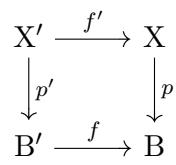
\includegraphics[keepaspectratio]{images/part001_4552bd62.jpg}}

of commutative squares; consider the square

\begin{enumerate}
\def\labelenumi{(\arabic{enumi})}
\setcounter{enumi}{13}
\tightlist
\item
\end{enumerate}

\pandocbounded{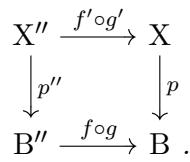
\includegraphics[keepaspectratio]{images/part001_1603e4c4.jpg}}

It is commutative. If squares (12) and (13) are Cartesian, then so is square (14). If squares (13) and (14) are Cartesian, then so is square (12).

Square (14) is commutative, since we have \(p \circ f' \circ g' = f \circ p' \circ g' = f \circ g \circ p''\) . Denote by \(h' : X'' \to B'' \times_{B'} X'\) , \(h : X' \to B' \times_{B} X\) and \(h'' : X'' \to B'' \times_{B} X\) the canonical continuous maps deduced from the commutative squares (12), (13), and (14). Moreover, denote

\[
j \colon \mathrm{B} ^ {\prime \prime} \times_ {\mathrm{B}} \mathrm{X} \rightarrow \mathrm{B} ^ {\prime \prime} \times_ {\mathrm{B} ^ {\prime}} (\mathrm{B} ^ {\prime} \times_ {\mathrm{B}} \mathrm{X})
\]

the continuous map that sends \((b'', x)\) to \((b'', g(b''), x)\) . It is a homeomorphism and one has \(j \circ h'' = (\mathrm{Id}_{\mathrm{B}''} \times_{\mathrm{B}} h) \circ h'\) .

Suppose that square (13) is Cartesian. Then h is a homeomorphism (I, p. 8, prop 2), so the map \(Id_{B''} \times_{B} h\) is a homeomorphism, and \(h''\) is a homeomorphism if and only if \(h'\) is one. This means that square (12) is Cartesian if and only if square (14) is Cartesian (loc. cit.).

With the notation of Proposition 7, one sometimes says that square (14) is the composite square of squares (13) and (12). The first assertion expresses that the composite of two Cartesian squares is Cartesian. In particular, the B''-spaces \(g^{*}(f^{*}(\mathrm{X}))\) and \((f \circ g)^{*}(\mathrm{X})\) are isomorphic.

\pandocbounded{
\includegraphics[keepaspectratio]{images/part001_52f28a70.jpg}}

Remarks. --- 1) It can happen that the squares (12) and (14) are Cartesian without the square (13) being so (I, p. 139, exerc. 2).

\begin{enumerate}
\def\labelenumi{\arabic{enumi})}
\setcounter{enumi}{1}
\tightlist
\item
  Let \(p \colon \mathrm{X} \to \mathrm{B}\) and \(f \colon \mathrm{B}' \to \mathrm{B}\) be continuous maps. The map \(g \colon \mathrm{B}' \to \mathrm{B}' \times \mathrm{B}\) defined by \(g(b') = (b', f(b'))\) is a homeomorphism from \(\mathrm{B}'\) onto the graph \(\mathrm{G}\) of the map \(f\) (TG, I, p. 25, cor. 2), and the fibered product \(\mathrm{B}' \times_{\mathrm{B}} \mathrm{X}\) is identified (I, p. 6) with the subspace of \(\mathrm{B}' \times \mathrm{X}\) that is the inverse image of \(\mathrm{G}\) under the map \(\mathrm{Id}_{\mathrm{B}'} \times p \colon \mathrm{B}' \times \mathrm{X} \to \mathrm{B}' \times \mathrm{B}\) . By the example of I, p. 10 and Corollary 1 of Proposition 5 (I, p. 11), the squares
\end{enumerate}

\[
\begin{array}{c c} \mathrm {B^ {\prime}} \times_ {\mathrm{B}} \mathrm{X} \xrightarrow {i} \mathrm {B^ {\prime}} \times \mathrm{X} & \mathrm {B^ {\prime}} \times \mathrm{X} \xrightarrow {\mathrm{pr} _ {2}} \mathrm{X} \\ \Biggl \downarrow \mathrm{pr} _ {1} & \Biggl \downarrow \mathrm{Id} _ {\mathrm {B^ {\prime}}} \times p \\ \mathrm {B^ {\prime}} \xrightarrow {g} \mathrm {B^ {\prime}} \times \mathrm{B} & \text {et} \end{array} \qquad \qquad \begin{array}{c c} \mathrm {B ^ {\prime}} \times \mathrm{X} \xrightarrow {\mathrm{pr} _ {2}} \mathrm{X} \\ \Biggl \downarrow \mathrm{Id} _ {\mathrm {B^ {\prime}}} \times p & \Biggl \downarrow p \\ \mathrm {B^ {\prime}} \times \mathrm{B} \xrightarrow {\mathrm{pr} _ {2}} \mathrm{B} & \end{array}
\]

(where i denotes the canonical injection) are Cartesian, and the Cartesian square

\[
\begin{array}{c} \mathrm{B} ^ {\prime} \times_ {\mathrm{B}} \mathrm{X} \xrightarrow {\mathrm{pr} _ {2}} \mathrm{X} \\ \Big \downarrow \mathrm{pr} _ {1} \\ \mathrm{B} ^ {\prime} \xrightarrow {f} \mathrm{B} \end{array}
\]

is their composite. In other words, every Cartesian square is identified with the composite square of a Cartesian square obtained by taking a product (I, p. 11, Corollary 1 of Proposition 5, square (8)) and a Cartesian square obtained by passing to subspaces (I, p. 10, example, square (5)).

\begin{enumerate}
\def\labelenumi{\arabic{enumi})}
\setcounter{enumi}{2}
\tightlist
\item
  Let
\end{enumerate}

\[
\begin{array}{c} \mathrm{X} _ {1} \xrightarrow {g _ {1}} \mathrm{X} \\ \Biggl \downarrow p _ {1} \\ \mathrm{B} _ {1} \xrightarrow {f _ {1}} \mathrm{B} \end{array}\tag{15}
\]

and

\[
\begin{array}{c} \mathrm{X} _ {2} \xrightarrow {g _ {2}} \mathrm{X} \\ \Biggl \downarrow p _ {2} \\ \mathrm{B} _ {2} \xrightarrow {f _ {2}} \mathrm{B} \end{array}\tag{16}
\]

  Let

\[
\begin{array}{c} \mathrm{X} _ {1} \times_ {\mathrm{X}} \mathrm{X} _ {2} \xrightarrow {g} \mathrm{X} \\ \Big \downarrow^ {p ^ {\prime}} \\ \mathrm{B} _ {1} \times_ {\mathrm{B}} \mathrm{B} _ {2} \xrightarrow {f} \mathrm{B} \end{array}\tag{17}
\]

where \(f\) (resp. \(g\) ) is the map that defines the structure of a B-space (resp. of an X-space) on the fibered product \(\mathrm{B}_{1} \times_{\mathrm{B}} \mathrm{B}_{2}\) (resp. on the fibered product \(\mathrm{X}_{1} \times_{\mathrm{X}} \mathrm{X}_{2}\) ) and where \(p'\) is the map induced by \(p_{1} \times p_{2}\) by passing to subspaces. It is Cartesian (I, p. 13, Corollary 2 of Proposition 5).

Now consider the following two commutative squares:

\[
\begin{array}{c c} \mathrm{X} _ {1} \times_ {\mathrm{X}} \mathrm{X} _ {2} \xrightarrow {\operatorname{pr} _ {1}} \mathrm{X} _ {1} & \mathrm{X} _ {1} \times_ {\mathrm{X}} \mathrm{X} _ {2} \xrightarrow {\operatorname{pr} _ {2}} \mathrm{X} _ {2} \\ \Biggl \downarrow p ^ {\prime} & \text {and} \\ \mathrm{B} _ {1} \times_ {\mathrm{B}} \mathrm{B} _ {2} \xrightarrow {\operatorname{pr} _ {1}} \mathrm{B} _ {1} & \mathrm{(19)} \\ & \mathrm{B} _ {1} \times_ {\mathrm{B}} \mathrm{B} _ {2} \xrightarrow {\operatorname{pr} _ {2}} \mathrm{B} _ {2}. \end{array}\tag{18}
\]

Square (17) is composed of squares (15) and (18), as well as squares (16) and (19). By prop. 7, squares (18) and (19) are Cartesian.

\subsection{Strict maps}

PROPOSITION 8. --- Let

\[
\begin{array}{c} \mathrm {X^ {\prime}} \xrightarrow {f ^ {\prime}} \mathrm{X} \\ \Big \downarrow_ {p ^ {\prime}} \\ \mathrm {B^ {\prime}} \xrightarrow {f} \mathrm{B} \end{array}
\]

a Cartesian square. If the map p is open (resp. is proper, resp. has a continuous section in a neighborhood of every point), then so is \(p'\).

By Remark 2, I, p. 16, it suffices to prove the proposition for Cartesian squares of the following type:

\[
\begin{array}{c c} \overline {{p}} ^ {1} (\mathrm {A}) \xrightarrow {j} \mathrm{X} & \mathrm {A} \times \mathrm{F} \xrightarrow {i} \mathrm{X} \times \mathrm{F} \\ \Big \downarrow_ {p _ {\mathrm {A}}} & \Big \downarrow_ {p \times \mathrm {Id}_{\mathrm {F}}} \\ \mathrm {A} & \xrightarrow {i} \mathrm {B} \end{array} \quad\text {and} \quad \begin{array}{c} \mathrm {X} \times \mathrm {F} \xrightarrow {j} \mathrm {X} \\ \Big \downarrow_ {p \times \mathrm {Id}_{\mathrm {F}}} \\ \mathrm {B} \times \mathrm {F} \xrightarrow {i} \mathrm {B} \end{array}
\]

where F is a topological space, A is a subspace of B, and i and j are the canonical injections. If the map p is open, the maps \(p_{A}\) and \(p \times Id_{F}\) are open (TG, I, p. 30, prop. 2 and TG, I, p. 34, prop. 8). If the map p is proper, then the maps \(p_{A}\) and \(p \times Id_{F}\) are proper (TG, I, p. 72, prop. 3 and TG, I, p. 72, def. 1). If U is an open subset of B and \(s\colon\mathrm{U}\to\mathrm{X}\) is a continuous section of p on U, the map \(s\mid(\mathrm{A}\cap\mathrm{U})\) is a continuous section of \(p_{\mathrm{A}}\) onto \(\mathrm{A}\cap\mathrm{U}\), and the map \(s\times\mathrm{Id}_{\mathrm{F}}\) is a continuous section of \(p\times\mathrm{Id}_{\mathrm{F}}\) onto \(\mathrm{U}\times\mathrm{F}\).

Remark 1. --- With the notation of Proposition 8, if \(p\) is a closed map, it is not necessarily the case that \(p'\) is closed (cf. TG, I, p. 32, prop. 3). However, if \(p\) is a map with a continuous section, \(p'\) also has a continuous section.

DEFINITION 5. --- Let X and Y be topological spaces and let f: X → Y be a map. Let R be the equivalence relation associated with f and

\[
\mathrm{X} \rightarrow \mathrm{X} / \mathrm{R} \xrightarrow {g} f (\mathrm{X}) \rightarrow \mathrm{Y}
\]

the canonical decomposition of \(f\) (E, II, p. 44). We say that the map \(f\) is strict if \(g\) is a homeomorphism, when \(X/R\) is equipped with the quotient topology and \(f(X)\) is equipped with the topology induced by that of \(Y\).

A strict map is continuous.

Recall (TG, I, p. 22, prop. 8) that for a map \(f\) to be strict, it is necessary and sufficient that \(f\) be continuous and that, for every subset \(A\) of \(X\) which is open (resp. closed) and saturated, \(f(A)\) be open (resp. closed) in \(f(X)\).

Examples. --- 1) The composition of two strict maps is not necessarily strict. Indeed, every continuous map \(f \colon X \to Y\) is the composite of the map \(\mathrm{pr}_2 \colon X \times Y \to Y\) and the map \(x \mapsto (x, f(x))\) from \(X\) into \(X \times Y\), both of which are strict (TG, I, p. 26, prop. 5 and TG, I, p. 25, cor. 2). On the other hand, the composite of two strict and injective (resp. surjective) maps is a strict map.

\begin{enumerate}
\def\labelenumi{\arabic{enumi})}
\setcounter{enumi}{1}
\item
  A continuous map that is open, or closed, or has a continuous section, is strict. This follows from Prop. 3 of TG, I, p. 32 and Prop. 9 of TG, I, p. 22.
\item
  For a continuous homomorphism from one topological group to another to be a strict morphism (TG, III, p. 16, def. 1), it is necessary and sufficient that it be a strict map in the sense of Definition 5.
\end{enumerate}

PROPOSITION 9. --- Let X, Y, and Z be topological spaces. Let \(f\colon X \to Y\) be a continuous surjective map and \(g\colon Y \to Z\) a map.

\begin{enumerate}
\def\labelenumi{\alph{enumi})}
\item
If f is strict and if g∘f is continuous, then the map g is continuous.
\item
If g is continuous and if g∘f is strict, then g is strict.
\item
If f and g \(\circ\) f are strict, then g is strict.
\end{enumerate}

Let us prove assertion a). Let R denote the relation associated with f in X; by hypothesis, the map from X/R onto Y induced by f by passing to the quotient is a homeomorphism. The first assertion then follows from Proposition 6 of I, p. 21.

Let us prove b). Let B be a closed saturated subset of Y for the relation defined by g, and let \(A = f^{-1}(B)\). Since f is continuous, A is closed in X, and A is saturated for the equivalence relation defined by \(g \circ f\). Since \(g \circ f\) is strict and f is surjective, \(g(B) = g \circ f(A)\) is then closed in Z. The continuous map g is therefore strict.

Assertion c) follows immediately from assertions a) and b).

PROPOSITION 10. --- Let X be a topological space and let R be an equivalence relation on X. Let Y be a locally compact topological space. Let S be the equivalence relation on X × Y which is the product of the equivalence relation R on X and the equality relation on Y. The canonical bijection (X × Y)/S → (X/R) × Y is a homeomorphism.

Recall that if U and V are topological spaces, \(\mathcal{C}_{c}(\mathrm{U};\mathrm{V})\) denotes the set of continuous maps from U to V, endowed with the compact-open topology (TG, X, p. 26, def. 1).

Let \(p \colon \mathrm{X} \to \mathrm{X} / \mathrm{R}\) and \(q \colon \mathrm{X} \times \mathrm{Y} \to (\mathrm{X} \times \mathrm{Y}) / \mathrm{S}\) be the canonical surjections. Let \(g \colon (\mathrm{X} \times \mathrm{Y}) / \mathrm{S} \to (\mathrm{X} / \mathrm{R}) \times \mathrm{Y}\) be the canonical bijection. It is continuous; let us denote its inverse by \(h\) and prove that it is continuous.

The map \(i\colon X \to \mathcal{C}_{c}(Y;X \times Y)\) such that, for every \(x \in X\), \(i(x)\) is the map defined by \(y \mapsto (x,y)\), is continuous (TG, X, p. 28, Theorem 3). The map \(\widetilde{q}\colon \mathcal{C}_{c}(Y;X \times Y) \to \mathcal{C}_{c}(Y;(X \times Y)/S)\), which associates to a continuous map \(\varphi\) the map \(q \circ \varphi\), is continuous (TG, X, p. 29, Proposition 9). Consequently, the map \(\widetilde{q} \circ i\colon X \to \mathcal{C}_{c}(Y;(X \times Y)/S)\) is continuous. It is compatible with the equivalence relation R; the unique map \(j\colon X/R \to \mathcal{C}_{c}(Y;(X \times Y)/S)\) such that \(j \circ p = \widetilde{q} \circ i\) is therefore continuous. We have \(h(\xi,y) = j(\xi)(y)\) for every pair \((\xi,y) \in (X/R) \times Y\). Since Y is locally compact, it follows from TG, X, p. 28, Theorem 3 that \(h\) is continuous.

The conclusion of Proposition 10 is no longer necessarily valid if Y is not locally compact (TG, I, p. 96, exerc. 6).

COROLLARY. --- Let X and Y be topological spaces and let \(f: X \to Y\) be a continuous map. Let T be a locally compact topological space. If the map f is strict, then so is the map \(f \times Id_{T}\) from \(X \times T\) into \(Y \times T\).

\subsection{Universally strict maps}

Let

\[
\begin{array}{c} \mathrm {X^ {\prime}} \xrightarrow {f ^ {\prime}} \mathrm{X} \\ \Big \downarrow_ {p ^ {\prime}} \\ \mathrm {B^ {\prime}} \xrightarrow {f} \mathrm{B} \end{array}
\]

a Cartesian square, where p is strict. The map \(p'\) is not necessarily strict (cf. Remark 1). However, if A is open (resp. closed) in B, the map \(p_A: \overline{p}^{1}(A) \to A\) is strict.

DEFINITION 6. --- Let p: X → B be a map. We say that p is universally strict if, for every Cartesian square

\pandocbounded{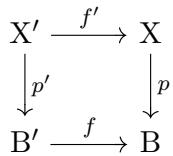
\includegraphics[keepaspectratio]{images/part001_50963eb1.jpg}}

the map p' is strict.

A universally strict map is strict. With the notation of Definition 6, if \(p\) is universally strict, then \(p'\) is universally strict as well. This follows immediately from the definition.

COROLLARY. --- An open map, a proper map, and a map having a continuous local section are universally strict.

Example. --- Let B be a topological space and \((\mathrm{A}_{i})_{i\in\mathrm{I}}\) a covering of B; we denote by A the sum space of the family \((\mathrm{A}_{i})_{i\in\mathrm{I}}\), and \(p: A \to B\) the canonical map. The map p is universally strict under each of the following two hypotheses:

\begin{enumerate}
\def\labelenumi{(\roman{enumi})}
\item
  For every point \(b \in B\) , there exists \(i \in I\) such that b is an interior point of \(A_{i}\) ;
\item
  The family \((A_{i})\) is locally finite and the \(A_{i}\) are closed subsets of B.
\end{enumerate}

Under hypothesis (i), the map p has a continuous section in a neighborhood of every point. Under hypothesis (ii), the map p is proper by definition of the sum space (resp. by TG, I, p. 6, prop. 4 and TG, I, p. 75, th. 1). It is therefore universally strict.

Remark. --- A closed map is not necessarily universally strict (cf. TG, I, p. 96, exerc. 6).

PROPOSITION 11. --- Let

\pandocbounded{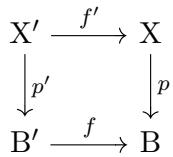
\includegraphics[keepaspectratio]{images/part001_02f1b349.jpg}}

a Cartesian square.

\begin{enumerate}
\def\labelenumi{\alph{enumi})}
\item
Suppose f is strict and surjective. Then, if p' is open (resp. closed, resp. proper), so is p.
\item
Suppose f is closed and surjective. If p' is strict, then p is strict.
\item
Suppose f is universally strict. If p' is universally strict, then p is universally strict.
\end{enumerate}

Note first that for every subset A of X, we have

\[
p ^ {\prime} ((\stackrel {- 1} {f ^ {\prime}}) (\mathrm{A})) = \stackrel {- 1} {f} (p (\mathrm{A})).\tag{20}
\]

Indeed, if \(x' \in (f')^{-1}(\mathrm{A})\), then \(f(p'(x')) = p \circ f'(x') \in p(\mathrm{A})\). Conversely, if \(b' \in f^{-1}(p(\mathrm{A}))\), let \(x \in A\) be such that \(f(b') = p(x)\). By definition of a Cartesian square, there exists a unique \(x' \in X'\) such that \(f'(x') = x\) and \(p'(x') = b'\), so that \(b' \in p'((f')^{-1}(\mathrm{A}))\).

Suppose that f is an open map and \(p'\) is a strict map.

The set \((f')^{-1}(\mathrm{A})\) is open (resp. closed) in \(\mathrm{X}'\). Consequently, the set \(p'((f')^{-1}(\mathrm{A}))\) is open (resp. closed) in \(\mathrm{B}'\). By relation (20), it is also saturated for the equivalence relation defined by \(f\). Since the map \(f\) is assumed to be surjective, we then have \(p(\mathrm{A}) = f(p'((f')^{-1}(\mathrm{A})))\), and since it is strict, the set \(p(\mathrm{A})\) is open (resp. closed) in B. The map \(p\) is therefore open (resp. closed).

For a continuous map to be proper, it is necessary and sufficient that it be closed and that its fibers be quasi-compact (TG, I, p. 75, th. 1). If the map \(p'\) is proper, the map \(p\) is closed by what precedes. Let us study its fibers: if \(b \in B\), let \(b' \in B'\) be such that \(f(b') = b\). By the corollary of I, p. 10, the map \(f'\) induces a homeomorphism \(X_{b'}' \to X_b\). Since \(p'\) is proper, \(X_{b'}'\) is quasi-compact, hence \(X_b\) is also. The map \(p\) is therefore proper.

Let us prove b) and c). Set \(Y = p(X)\) and \(Y' = p'(X')\). Relation (20) applied to X implies that \(Y' = f^{-1}(Y)\). Let g denote the map from \(Y'\) into Y induced by f. In case b), the map g is strict by Remark 1, I, p. 18. In case c), it is strict by Definition 6 since the square

\pandocbounded{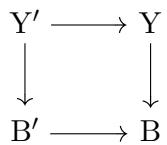
\includegraphics[keepaspectratio]{images/part001_f35053b2.jpg}}

is Cartesian.

Denote by \(q\) and \(q'\) the maps from X to Y and from \(X'\) to \(Y'\), respectively, induced by the maps \(p\) and \(p'\).

\[
\begin{array}{c} \mathrm {X^ {\prime}} \xrightarrow {f ^ {\prime}} \mathrm{X} \\ \Big \downarrow q ^ {\prime} \\ \mathrm {Y^ {\prime}} \xrightarrow {g} \mathrm{Y} \end{array}
\]

Since \(f\) is surjective, \(f'\) is also surjective; by Proposition 9 b), \(p\) is strict.

COROLLARY 1. --- Suppose that the map f is universally strict and surjective and that the map p' is universally strict. Then the map p is universally strict.

Let

\[
\begin{array}{c} \mathrm{Y} \xrightarrow {g ^ {\prime}} \mathrm{X} \\ \Biggl \downarrow q \\ \mathrm{C} \xrightarrow {g} \mathrm{B} \end{array}
\]

a Cartesian square; the goal is to prove that the map q is strict. By Remark 3 of I, p. 16, the squares

\[
\begin{array}{c} \mathrm {X^ {\prime}} \times_ {\mathrm{X}} \mathrm{Y} \xrightarrow {\mathrm{pr} _ {1}} \mathrm {X^ {\prime}} \\ \Biggl \downarrow r \\ \mathrm {B^ {\prime}} \times_ {\mathrm{B}} \mathrm{C} \xrightarrow {\mathrm{pr} _ {1}} \mathrm {B^ {\prime}} \end{array}
\]

and

\[
\begin{array}{c} \mathrm {X^ {\prime} \times_ {X} Y\xrightarrow {pr_ {2}} Y} \\ \Big \downarrow r \\ \mathrm {B^ {\prime} \times_ {B} C\xrightarrow {pr_ {2}} C} \end{array}\tag{21}
\]

are Cartesian, where \(r \colon X' \times_{X} Y \to B' \times_{B} C\) denotes the map induced by \((p', q)\). As the map \(f\) is universally strict and surjective, the same holds for the map \(\mathrm{pr}_2 \colon B' \times_{B} C \to C\) (I, p. 20, def. 6 and I, p. 10, cor. of prop. 4). On the other hand, the map \(r\) is strict, since \(p'\) is assumed to be universally strict. By Proposition 11, c) applied to the Cartesian square (21), the map \(q\) is strict.

COROLLARY 2. --- Let B and X be topological spaces and let \(p\colon X \to B\) be a continuous map. Let \((A_i)_{i \in I}\) be a family of subsets of B that is an open cover of B, or else a locally finite closed cover of B. If for every \(i \in I\), the map \(p_{A_i}\colon \overline{p}^1(A_i) \to A_i\) is strict (resp. universally strict), the map p is strict (resp. universally strict).

For every \(i \in \mathrm{I}\), set \(\mathrm{Y}_i = \overline{p}^{1}(\mathrm{A}_i)\) and \(p_i = p_{\mathrm{A}_i}\). Let A be the sum space of the family \((\mathrm{A}_i)_{i \in \mathrm{I}}\) and Y the sum space of the family \((\mathrm{Y}_i)_{i \in \mathrm{I}}\); let us denote by \(f: \mathrm{A} \to \mathrm{B}\) (resp. \(g: \mathrm{Y} \to \mathrm{X}\), \(q: \mathrm{Y} \to \mathrm{A}\)) the map induced by the family of canonical injections \(A_i \rightarrow B\) (resp. of canonical injections \(Y_i \rightarrow X\) and of the maps \(p_i\)). The square

\[
\begin{array}{c} \mathrm{Y} \xrightarrow {g} \mathrm{X} \\ \Big \downarrow q \\ \mathrm{A} \xrightarrow {f} \mathrm{B} \end{array}
\]

is a Cartesian square (Examples, I, p. 10 and p. 14). By the corollary, I, p. 20, the map \(f\) is universally strict. By Proposition 11, it therefore suffices to prove that the map \(q\) is strict (resp. universally strict) if the maps \(p_i\), for \(i \in I\), are strict (resp. universally strict). We are thus reduced to proving the corollary when the sets \(A_i\), \(i \in I\), form a partition of the space B into open and closed parts, which we will henceforth assume.

Suppose that each of the maps \(p_i\), \(i \in I\), is strict. If U is an open subset of X and is saturated for the equivalence relation defined by p, the set \(p_i(\mathrm{X}_i \cap \mathrm{U})\) is open in \(\mathrm{A}_i\) and \(p(\mathrm{U}) = \bigcup_{i \in \mathrm{I}} p_i(\mathrm{X}_i \cap \mathrm{U})\) is open in B. The map p is therefore strict.

Suppose now that each of the maps \(p_{i}, i \in I\), is universally strict, and let us show that the map p is universally strict. Let C be a topological space and \(h: C \to B\) a continuous map. The goal is to show that the map \(pr_{1}: X \times_{B} C \to C\) is strict. The space C is identified with the sum space of the family \(C_{i} = h^{-1}(A_{i})\), and the space \(X \times_{B} C\) is identified with the direct sum space of the family \(X \times_{B} C_{i} = X_{i} \times_{A_{i}} C_{i}\). Since \(p_{i}\) is universally strict, the map \(pr_{1}: X_{i} \times_{A_{i}} C_{i} \to C_{i}\) is strict. By the preceding, the map \(pr_{1}: X \times_{B} C \to C\) is strict. This proves that the map p is universally strict.

\section{ÉTALE MAPS}

\subsection{Separated maps}

PROPOSITION 1. --- Let X and Y be topological spaces, and let \(f\colon X \to Y\) be a continuous map. The following properties are equivalent:

\begin{enumerate}
\def\labelenumi{(\roman{enumi})}
\item
  The diagonal \(\Delta_{X}\) of the fibered product X \(\times_{Y}\) X is a closed subspace;
\item
  For every topological space W and every pair of continuous maps \((g_{1}, g_{2})\) from W into X such that \(f \circ g_{1} = f \circ g_{2}\) , the set of points \(w \in W\) such that \(g_{1}(w) = g_{2}(w)\) is closed in W;
\item
  For every pair \((x_{1}, x_{2})\) of points of X such that \(x_{1} \neq x_{2}\) and \(f(x_{1}) = f(x_{2})\) , there exists a neighborhood \(V_{1}\) of \(x_{1}\) in X and a neighborhood \(V_{2}\) of \(x_{2}\) in X such that \(V_{1} \cap V_{2} = \varnothing\) .
\end{enumerate}

(i)⇒(ii): Let \(g_{1}\) and \(g_{2}\) be continuous maps from W into X such that \(f \circ g_{1} = f \circ g_{2}\), and let \(g: W \to X \times_{Y} X\) be the map induced by \(g_{1}\) and \(g_{2}\). The set of points \(w \in W\) such that \(g_{1}(w) = g_{2}(w)\) is \(g^{-1}(\Delta_{X})\). Since g is continuous, it is therefore closed if the diagonal \(\Delta_{X}\) is closed.

(ii)⇒(i): The diagonal \(\Delta_{X}\) is the set of points \(z \in X \times_{Y} X\) such that \(\mathrm{pr}_{1}(z) = \mathrm{pr}_{2}(z)\). It follows from (ii), applied to \(W = X \times_{Y} X\) and to the pair of maps \((\mathrm{pr}_{1}, \mathrm{pr}_{2})\), that the diagonal \(\Delta_{X}\) is closed in \(X \times_{Y} X\).

(i)⇔(iii): Let \((x_{1}, x_{2})\) be a point of \(X \times_{Y} X\) and let \(V_{1}\) and \(V_{2}\) be neighborhoods of \(x_{1}\) and \(x_{2}\), respectively. The condition \(V_{1} \cap V_{2} = \varnothing\) is equivalent to the condition \((\mathrm{V}_{1} \times \mathrm{V}_{2}) \cap \Delta_{\mathrm{X}} = \varnothing\), that is, to \((\mathrm{V}_{1} \times \mathrm{V}_{2}) \cap (\mathrm{X} \times_{\mathrm{Y}} \mathrm{X}) \cap \Delta_{\mathrm{X}} = \varnothing\). Since the sets \((\mathrm{V}_{1} \times \mathrm{V}_{2}) \cap (\mathrm{X} \times_{\mathrm{Y}} \mathrm{X})\) form a base of neighborhoods of \((x_{1}, x_{2})\) in \(X \times_{Y} X\), this proves the equivalence of (i) and (iii).

DEFINITION 1. --- Let X and Y be topological spaces. A continuous map \(f: X \to Y\) is separated if it satisfies the equivalent conditions of Proposition 1.

PROPOSITION 2. --- Let X, Y, Z be topological spaces and let \(f\colon X \to Y\) and \(g\colon Y \to Z\) be continuous maps.

\begin{enumerate}
\def\labelenumi{\alph{enumi})}
\item
  If f and g are separated, then \(g \circ f\) is separated.
\item
If g \(\circ\) f is separated, then f is separated.
\item
  Suppose further that the map f is proper and surjective. Then, if g ∘ f is separated, g is separated.
\end{enumerate}

Consider, in X×X, the subspaces \(\Delta_{X}\) (diagonal), \(X \times_Y X\) and \(X \times_Z X\). These are respectively the sets of points u of X×X such that \(\mathrm{pr}_{1}(u)=\mathrm{pr}_{2}(u)\), \(f\circ\mathrm{pr}_{1}(u)=f\circ\mathrm{pr}_{2}(u)\), \(g\circ f\circ\mathrm{pr}_{1}(u)=g\circ f\circ\mathrm{pr}_{2}(u)\). If \(g\circ f\) is separated, \(\Delta_{X}\) is closed in \(X \times_Z X\), hence also in \(X \times_Y X\), whence b).

By Proposition 1, (ii), applied to W = X ×\_Z X, \(g_1 = f \circ \text{pr}_1\) and \(g_2 = f \circ \text{pr}_2\), X ×\_Y X is closed in X ×\_Z X if \(g\) is separated. If moreover \(f\) is separated, \(\Delta_X\) is closed in X ×\_Y X (Proposition 1, (i)), hence in X ×\_Z X, whence \(a\).

Finally, let us prove \(c\). The map \((f, f) \colon X \times X \to Y \times Y\) is proper (TG, I, p. 73, prop. 4). The subspace \(X \times_Z X\) is the inverse image of \(Y \times_Z Y\) under \((f, f)\); by TG, I, p. 72, prop. 3, the map \(u \colon X \times_Z X \to Y \times_Z Y\) induced by \((f, f)\) is proper. Since \(g \circ f\) is separated, the diagonal \(\Delta_X\) is closed in \(X \times_Z X\). Consequently, \(u(\Delta_X)\) is closed in \(Y \times_Z Y\). Since \(f\) is surjective, \(u(\Delta_X)\) is the diagonal of \(Y \times_Z Y\). This shows that \(g\) is separated.

Remarks. --- 1) An injective continuous map is separated.

\begin{enumerate}
\def\labelenumi{\arabic{enumi})}
\setcounter{enumi}{1}
\tightlist
\item
  For a topological space X to be Hausdorff (TG, I, p. 52, def. 1), it is necessary and sufficient that the map from X into a space reduced to a single point be separated. In this case, every continuous map from X into a topological space is separated (Proposition 1, (iii)).
\end{enumerate}

Let \(f\colon X \to Y\) be a continuous and separated map. For every point \(y\) of \(Y\), the fiber \(f^{-1}(y)\) is a separated topological space (loc. cit.). There nevertheless exist continuous maps which are not separated but all of whose fibers are separated topological spaces (I, p. 140, exerc. 1).

\begin{enumerate}
\def\labelenumi{\arabic{enumi})}
\setcounter{enumi}{2}
\item
  Let \(f \colon X \to Y\) be a continuous and separated map. If the space Y is separated, then the space X is separated. This follows from Remark 2 and Proposition 2 applied with a space Z reduced to a point.
\item
  Let \(f \colon X \to Y\) be a continuous and separated map, let \(y\) be a point of \(Y\), and let \(A\) be a finite subset of \(f^{-1}(y)\). Let us prove that there exists a family \((V_a)_{a \in A}\) of pairwise disjoint sets such that, for each \(a \in A\), the set \(V_a\) is a neighborhood of \(a\) in X. To do this, for each subset \(\{a,b\}\) of \(A\) with two elements, choose a neighborhood \(V_{(a,b)}\) of \(a\) and a neighborhood \(\mathrm{V}_{(b,a)}\) of \(b\) in X such that \(\mathrm{V}_{(a,b)} \cap \mathrm{V}_{(b,a)} = \varnothing\) (Proposition 1, (iii)). Let \(\mathrm{V}_a\) denote the intersection of the family formed by X and the sets \(\mathrm{V}_{(a,b)}\) for \(b \in \mathrm{A}\), \(b \neq a\). The set \(\mathrm{V}_a\) is a neighborhood of \(a\) in X, and if \(a\), \(b\) are two distinct elements of A, the set \(\mathrm{V}_a \cap \mathrm{V}_b\) is contained in \(\mathrm{V}_{(a,b)} \cap \mathrm{V}_{(b,a)}\), hence is empty.
\item
  Let \(Y\) be a topological space. Let \((\mathrm{A}_{i})_{i\in\mathrm{I}}\) be a family of subsets of Y and let X be the sum space of the family \((\mathrm{A}_{i})_{i\in\mathrm{I}}\). The canonical map from X to Y is separated.
\end{enumerate}

PROPOSITION 3. --- Let \(f\colon X \to Y\) be a continuous and separated map. Every continuous section of \(f\) induces a homeomorphism of \(Y\) onto a closed subset of \(X\).

Let \(s\colon Y \to X\) be a continuous section of \(f\). The map \(s\) induces a homeomorphism of \(Y\) onto the subspace \(s(Y)\) of \(X\) (TG, I, p. 22, prop. 9). The identity map of \(X\) and the map \(s \circ f\) are continuous and one has \(f \circ \mathrm {Id}_{X} = f \circ (s \circ f)\). Since the map \(f\) is separated, the set \(s(Y)\), which is the set of points \(x\) of \(X\) such that \(x = (s \circ f)(x)\), is closed in \(X\) (Proposition 1, (ii)).

PROPOSITION 4. --- Let

\pandocbounded{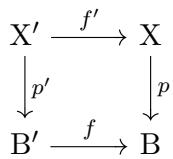
\includegraphics[keepaspectratio]{images/part001_94ec13ba.jpg}}

a Cartesian square. If the map p is separated, then so is p'. Conversely, if p' is separated and if f is universally strict and surjective, then p is separated.

Consider the square

\[
\begin{array}{c} \mathrm {X^ {\prime} \times_ {B^ {\prime}} X^ {\prime}} \xrightarrow {\varphi} \mathrm {X \times_ {B} X} \\ \Biggl \downarrow_ {q ^ {\prime}} \\ \mathrm {B^ {\prime} \xrightarrow {f} B} \end{array}
\]

where the map \(\varphi\) is induced by the map \(f' \times f': X' \times X' \to X \times X\) . Recall (I, p. 13, example 1) that this square is Cartesian and that one has \(\overline{\varphi}^1(\Delta_X) = \Delta_{X'}\) .

If the map p is separated, the set \(\Delta_{\mathrm{X}}\) is closed in \(\mathrm{X} \times_{\mathrm{B}} \mathrm{X}\); therefore, \(\Delta_{\mathrm{X}'}\) is a closed subset of \(\mathrm{X}' \times_{\mathrm{B}'} \mathrm{X}'\), which proves that the map \(p'\) is separated.

If the map f is surjective, the map \(\varphi\) is surjective (I, p. 10, cor.); if f is universally strict, \(\varphi\) is strict (I, p. 20, def. 6). Suppose the map \(p'\) is separated. Then \(\Delta_{\mathrm{X}'}\) is closed in \(\mathrm{X}' \times_{\mathrm{B}'} \mathrm{X}'\). Since \(\Delta_{\mathrm{X}'} = \overline{\varphi}^{1}(\Delta_{\mathrm{X}})\) and since \(\varphi\) is surjective and strict, \(\Delta_{\mathrm{X}}\) is closed in \(\mathrm{X} \times_{\mathrm{B}} \mathrm{X}\), which proves that the map \(p\) is separated.

PROPOSITION 5. --- Let \(f: X \to Y\) and \(g: Y \to Z\) be continuous maps. Suppose the map \(g\) is separated and the map \(g \circ f\) is proper. The map \(f\) is then proper.

Consider the following Cartesian square:

\[
\begin{array}{c} \mathrm{X} \times_ {\mathrm{Z}} \mathrm{Y} \xrightarrow {\operatorname{pr} _ {2}} \mathrm{Y} \\ \Biggl \downarrow \operatorname{pr} _ {1} \\ \mathrm{X} \xrightarrow {g \circ f} \mathrm{Z}. \end{array}
\]

Let \(s \colon X \to X \times_{Z} Y\) be the map \(x \mapsto (x, f(x))\). This is a continuous section of \(\mathrm{pr}_1 \colon X \times_{Z} Y \to X\). By Proposition 4, the map \(\mathrm{pr}_1\) is separated; it follows that the map \(s\) is proper (I, p. 27, prop. 3 and TG, I, p. 72, prop. 2). On the other hand, the map \(\mathrm{pr}_2\) is proper (I, p. 17, prop. 8). Therefore the map \(f\), which is equal to \(\mathrm{pr}_2 \circ s\), is proper (TG, I, p. 73, prop. 5).

\subsection{Étale maps}

DEFINITION 2. --- Let E and B be topological spaces, let \(p\colon\mathrm{E}\to\mathrm{B}\) be a map and let \(x\) be a point of E. One says that the map \(p\) is topologically étale at \(x\) if there exists a neighborhood U of \(x\) in E and a neighborhood V of \(p(x)\) in B such that \(p\) induces a homeomorphism from U onto V.

One says that the map p is topologically étale if it is topologically étale at every point x of E.

When there is no possible confusion (cf. Example 3 below), one says étale instead of topologically étale. Instead of saying that \(p\colon \mathrm{E}\to \mathrm{B}\) is an étale map, one also says that the B-space \((\mathrm{E},p)\) is an étale B-space, or simply that E is an étale space over B, when no doubt is possible as to the map \(p\).

Remarks. --- 1) The set of points of E at which a map \(p \colon \mathrm{E} \to \mathrm{B}\) is étale is an open subset U of E and the restriction of p to U is an étale map from U to B.

\begin{enumerate}
\def\labelenumi{\arabic{enumi})}
\setcounter{enumi}{1}
\tightlist
\item
  An étale map is continuous and open (TG, I, p. 33, prop. 5); in particular, the image of an étale map is open. Conversely, if \(p \colon \mathrm{E} \to \mathrm{B}\) is a continuous and open mapping, and if every point x of E has a neighborhood V such that the map \(p \mid \mathrm{V}\) is injective, the map p is étale. The fibers of an étale map are discrete.
\end{enumerate}

Examples. --- 1) Let B be a topological space and \((\mathrm{U}_{i})_{i\in\mathrm{I}}\) a family of subsets of B. Let E denote the sum space of the family \((\mathrm{U}_{i})_{i\in\mathrm{I}}\) and \(p: E \to B\) the map induced by the canonical injections of the \(U_{i}\) in B. For the map p to be étale, it is necessary and sufficient that the \(U_{i}\), \(i \in I\), all be open.

\begin{enumerate}
\def\labelenumi{\arabic{enumi})}
\setcounter{enumi}{1}
\item
For a holomorphic function \(f\colon U \to \mathbf{C}\) to be an étale map, it is necessary and sufficient that its derivative does not vanish.
\item
  An étale morphism of varieties (VAR, R, 5.7.8) is a topologically étale map, but there exist morphisms of real varieties that are topologically étale and are not étale morphisms. This is the case, for example, of the map \(x \mapsto x^3\) from \(\mathbf{R}\) into \(\mathbf{R}\). However, a morphism of complex analytic varieties that is topologically étale is an étale morphism (I, p. 141, exerc. 6).
\end{enumerate}

PROPOSITION 6. — Let X, Y, Z be topological spaces and let \(f\colon X\to Y\) , \(g\colon Y\to Z\) be maps.

\begin{enumerate}
\def\labelenumi{\alph{enumi})}
\item
  Suppose that f and g are étale; then \(g \circ f\) is étale.
\item
  Suppose that \(g\) is étale, \(f\) is continuous and \(g \circ f\) is open. Then \(f\) is open.
\item
  Suppose that \(g \circ f\) and \(g\) are étale and that \(f\) is continuous. The map \(f\) is then étale.
\item
  Suppose that \(g \circ f\) is étale and that the map \(f\) is continuous and open; then, \(f\) is étale and \(g\) is étale at every point of \(f(\mathrm{X})\) .
\end{enumerate}

Let us prove (a). Suppose that \(f\) and \(g\) are étale. They are then continuous and open, so the map \(g \circ f\) is continuous and open. Let \(x\) be a point of X. There exists a neighborhood W of \(f(x)\) in Y such that \(g \mid \mathrm{W}\) is injective, and a neighborhood V of \(x\) in X, contained in \(f(\mathrm{W})\), such that \(f \mid \mathrm{V}\) is injective; the map \((g \circ f) \mid \mathrm{V}\) is then injective. This proves that the map \(g \circ f\) is étale (Remark 2).

Let us prove b). Let x be a point of X and W an open neighborhood of \(f(x)\) such that g induces a homeomorphism from W onto the open set \(g(\mathrm{W})\). Let V be a neighborhood of x such that \(f(\mathrm{V})\) is contained in W; then, \(g \circ f(\mathrm{V})\) is a neighborhood of \(g \circ f(x)\), therefore \(f(\mathrm{V})\) is a neighborhood of \(f(x)\) in the open set W, and also in Y. This proves that the map f is open (TG, I, p. 33, prop. 5).

Let us prove c). By b), f is open. Let x be a point of X. Since \(g \circ f\) is étale, there exists a neighborhood V of x in X such that \(g \circ f \mid V\) is injective. Thus, \(f \mid V\) is injective and f is étale (I, p. 29, remark 2).

Let us prove d). Let \(x\) be a point of \(X\) and set \(y = f(x)\). There exists an open neighborhood \(V\) of \(x\) such that \(g \circ f\) induces a homeomorphism from \(V\) onto the open set \(g \circ f(V)\). As the map \(f\) is open, \(f(V)\) is an open neighborhood of \(y\). The map \(f|_V\colon V \to f(V)\) induced by \(f\) by passing to subspaces is continuous, open, and bijective; it is therefore a homeomorphism, so that \(f\) is étale at \(x\). Moreover, the map \(g\) induces a homeomorphism of \(f(V)\) onto \(g \circ f(V)\), hence is étale at \(y\).

COROLLARY 1. — Let B be a topological space. A B-morphism from one étale B-space to another is étale.

This follows from assertion c) of Prop. 6.

COROLLARY 2. --- Let B be a topological space; a bijective B-morphism from one étale B-space to another is a B-isomorphism.

By corollary 1, such a morphism is étale; it is therefore open (I, p. 29, remark 2). If it is bijective, it is a B-isomorphism.

COROLLARY 3. --- Let p: E → B be an étale map. Every continuous section of p induces a homeomorphism of B onto an open subset of E.

Indeed, such a section is étale (corollary 1), hence open.

COROLLARY 4. --- Let p: E → B be an étale and separated map. Suppose that E is connected and that p admits a section. Then p is a homeomorphism.

Let \(s\) be a section of \(p\) ; since \(p\) is étale, the image of \(s\) is open in E (Corollary 3); it is also closed, since \(p\) is separated (I, p. 27, prop. 3). Since E is connected, we have \(s(\mathrm{B}) = \mathrm{E}\) and \(p\) is a homeomorphism.

PROPOSITION 7. --- Let \(p\colon E \to B\) be a continuous map. For the map \(p\) to be étale, it is necessary and sufficient that it be open and that the diagonal \(\Delta_{E}\) of \(E \times_{B} E\) be open in \(E \times_{B} E\).

Suppose first that the map p is étale. Then it is open and every point of E has a neighborhood V such that \(p|V\) is injective, which amounts to saying that one has \((\mathrm{V} \times \mathrm{V}) \cap (\mathrm{E} \times_{\mathrm{B}} \mathrm{E}) \subset \Delta_{\mathrm{E}}\) . Therefore, \(\Delta_{E}\) is an open subset of \(E \times_{B} E\) .

Conversely, suppose that p is an open mapping and that \(\Delta_{\mathrm{E}}\) is an open subset of \(\mathrm{E} \times_{\mathrm{B}} \mathrm{E}\) . Let x be a point of E. Let V be an open neighborhood of x in E such that \((\mathrm{V} \times \mathrm{V}) \cap (\mathrm{E} \times_{\mathrm{B}} \mathrm{E})\) is contained in \(\Delta_{\mathrm{E}}\) . Then, \(p \mid \mathrm{V}\) is injective. By Remark 2, I, p. 29, the map p is étale.

PROPOSITION 8. --- Let

\pandocbounded{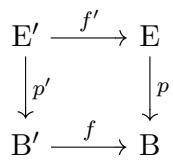
\includegraphics[keepaspectratio]{images/part001_e4ab0ebd.jpg}}

a Cartesian square. If the morphism p is étale, then the morphism p' is étale. Conversely, if the morphism p' is étale and the morphism f is universally strict and surjective, then the morphism p is étale.

Suppose that the map p is étale. In particular, it is open and \(p'\) is open (I, p. 17, prop. 8). Consider then the Cartesian square (I, p. 13, example 1)

\[
\begin{array}{c} \mathrm{E} ^ {\prime} \times_ {\mathrm{B} ^ {\prime}} \mathrm{E} ^ {\prime} \xrightarrow {\varphi} \mathrm{E} \times_ {\mathrm{B}} \mathrm{E} \\ \Biggl \downarrow q ^ {\prime} \qquad \qquad \qquad \qquad \Biggl \downarrow q \\ \mathrm{B} ^ {\prime} \xrightarrow {f} \mathrm{B}. \end{array}
\]

We have \(\Delta_{\mathrm{E}^{\prime}} = \overline{\varphi}^{1}(\Delta_{\mathrm{E}})\) (loc. cit.). Moreover, the diagonal \(\Delta_{\mathrm{E}}\) is open in \(\mathrm{E} \times_{\mathrm{B}} \mathrm{E}\) (prop. 7), hence the diagonal \(\Delta_{\mathrm{E}^{\prime}}\) is open in \(\mathrm{E}^{\prime} \times_{\mathrm{B}^{\prime}} \mathrm{E}^{\prime}\). This proves that the map \(p^{\prime}\) is étale (loc. cit.).

Suppose now that the map \(f\) is surjective and universally strict, and let the map \(p'\) be étale. Then, \(p'\) is open, therefore \(p\) is open (I, p. 21, prop. 11, \(a\)). On the other hand \(\Delta_{\mathrm{E}'}\) is an open subset of \(\mathrm{E}' \times_{\mathrm{B}'} \mathrm{E}'\). Since \(\Delta_{\mathrm{E}'} = \overline{\varphi}^{1}(\Delta_{\mathrm{E}})\) and the map \(\varphi\) is surjective and strict (I, p. 20, def. 6), \(\Delta_{\mathrm{E}}\) is open in \(\mathrm{E} \times_{\mathrm{B}} \mathrm{E}\). By prop. 7, the map p is étale.

COROLLARY. --- Let B be a topological space. The fiber product of two étale B-spaces is an étale B-space.

Let \((\mathrm{E}, p)\) and \((\mathrm{E}^{\prime}, p^{\prime})\) be étale B-spaces. The map \(pr_{1}: E \times_{B} E^{\prime} \to E\) is étale (prop. 8), hence the map \(p \circ pr_{1}: E \times_{B} E^{\prime} \to B\) is étale (prop. 6, a)).

Remark 3. --- Let

\pandocbounded{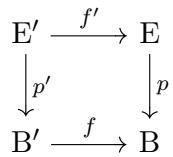
\includegraphics[keepaspectratio]{images/part001_b818a80c.jpg}}

a Cartesian square. If the map p is étale and the map f is strict, then the map \(f'\) is strict. Indeed, under these hypotheses, every point of E has an open neighborhood U such that p induces a homeomorphism from U onto the open set \(p(\mathrm{U})\) . The map \(p'\) induces then a homeomorphism of \((f')^{-1}(\mathrm{U})\) onto \(f^{-1}(p(\mathrm{U}))\). The map f induces a strict map from \(f^{-1}(p(\mathrm{U}))\) onto \(p(\mathrm{U})\) (I, p. 20) and the map \(f'\) therefore induces a strict map from \((f')^{-1}(\mathrm{U})\) into U. It follows that the map \(f'\) is strict (I, p. 23, corollary 2).

\subsection{Local sections of étale maps}

Let E and B be sets, A a subset of B, and \(p: E \rightarrow B\) a map. A section of p over A (or on A) is a map \(s: A \rightarrow E\) such that \(p \circ s\) is the canonical injection of A into B. The data of a section s of p over A is equivalent to the data of a section of the map \(p_{\mathrm{A}} \colon \overline{p}^{1}(\mathrm{A}) \to \mathrm{A}\) induced by p. If s is a section of p over A and if \(A'\) is a subset of A, the restriction \(s'\) of s to \(A'\) is a section of p over \(A'\). We then say that s is an extension of \(s'\) to A.

When E and B are topological spaces and \(p \colon \mathrm{E} \to \mathrm{B}\) is a continuous map, the set \(\mathcal{C}_{\mathrm{B}}(\mathrm{A};\mathrm{E})\) (I, p. 2) of continuous sections of \(p\) over A is also denoted by \(\mathcal{S}(\mathrm{A};p)\) or \(\mathcal{S}(\mathrm{A};\mathrm{E})\). Let \(s\) be a continuous section of \(p\) over A. The map \(s\) induces a homeomorphism of A onto \(s(\mathrm{A})\), and \(p\) induces the inverse homeomorphism. By Definition 2, I, p. 28, we therefore have:

PROPOSITION 9. --- Let p: E → B be a continuous map. For p to be étale, it is necessary and sufficient that every point of E have an open neighborhood which is the image of a continuous section of p over an open subset of B.

Remarks. --- 1) Let \(p \colon \mathrm{E} \to \mathrm{B}\) be a continuous and open map. For an open set U of E to be the image of a continuous section of \(p\) over an open set of B, it is necessary and sufficient that the restriction of \(p\) to U be injective.

\begin{enumerate}
\def\labelenumi{\arabic{enumi})}
\setcounter{enumi}{1}
\tightlist
\item
  Let \(p \colon \mathrm{E} \to \mathrm{B}\) a continuous map. Suppose that every point of B has an open neighborhood V such that there exists a continuous section of \(p\) over V. Such a map \(p\) is not necessarily étale, nor even open. It is nevertheless surjective and universally strict (I, p. 20, corollary).
\end{enumerate}

\subsection{Continuous liftings of étale maps}

Let \(p \colon \mathrm{E} \to \mathrm{B}\) and \(f \colon \mathrm{Z} \to \mathrm{B}\) be continuous maps. A continuous lifting of \(f\) to \(\mathrm{E}\) is called a continuous map \(g \colon \mathrm{Z} \to \mathrm{E}\) such that \(p \circ g = f\). The set of continuous liftings of \(f\) to \(\mathrm{E}\) is none other than \(\mathcal{C}_{\mathrm{B}}(\mathrm{Z};\mathrm{E})\). It is also identified with the set \(\mathcal{S}(\mathrm{Z};\mathrm{Z} \times_{\mathrm{B}}\mathrm{E})\) of continuous sections of the projection of the Z-space \((\mathrm{Z} \times_{\mathrm{B}}\mathrm{E},\mathrm{pr}_{1})\).

If T is a subset of Z, a continuous lifting of f to E defined on T is called a continuous lifting of f \textbar{} T to E:

\pandocbounded{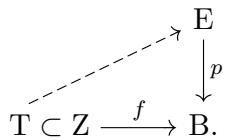
\includegraphics[keepaspectratio]{images/part001_46887bc2.jpg}}

PROPOSITION 10. --- Let E, B and Z be topological spaces, \(p\colon E \to B\) an étale map and \(f\colon Z \to B\) a continuous map.

Let \(z \in \mathbf{Z}\) and \(x \in \mathrm{E}\) be points such that \(f(z) = p(x)\). There exists a neighborhood \(\mathrm{W}\) of \(z\) on \(\mathbf{Z}\) and a continuous lifting \(g\) of \(f\) to \(\mathrm{E}\), defined on \(\mathrm{W}\), such that \(g(z) = x\).

There exists an open neighborhood V of \(p(x)\) in B and a continuous section s of p over V such that \(s(p(x)) = x\) (Proposition 9). The set \(W = f^{-1}(V)\) is an open neighborhood of z and the map \(g = s \circ (f|W)\) is a continuous lifting of f to E, defined on W and such that \(g(z) = x\).

PROPOSITION 11. --- Let E, B, and Z be topological spaces, let \(p\colon E \to B\) and \(f\colon Z \to B\) be continuous maps. Let \(g\) and \(g'\) be continuous liftings of \(f\) to E. Let W be the set of points of Z where \(g\) and \(g'\) coincide.

\begin{enumerate}
\def\labelenumi{\alph{enumi})}
\item
  If the map p is separated, W is closed.
\item
  If the map p is étale, W is open.
\end{enumerate}

Denote by \(h\) the continuous map \((g, g')\colon Z \to E \times E\). The image of \(h\) is contained in \(E \times_{B} E\) since \(p \circ g = f = p \circ g'\), and the set W of points of Z where g and g' coincide is the inverse image under \(h\) of the diagonal \(\Delta_{E}\).

If the map p is étale, the diagonal \(\Delta_{E}\) is open in \(E \times_{B} E\) (I, p. 31, prop. 7), hence the set W is open in Z.

If the map p is separated, the diagonal \(\Delta_{E}\) is closed in \(E \times_{B} E\) (I, p. 25, def. 1) and the set W is closed in Z.

COROLLARY 1. --- If the space Z is connected and if the map p is étale and separated, then continuous liftings of f to E that coincide at one point are equal.

COROLLARY 2. --- Let \(p\colon E \to B\) be a separated étale map. If the space E is connected, the group \(\mathrm{Aut}_{\mathrm{B}}(\mathrm{E})\) acts freely on E.

Indeed, if \(f: \mathrm{E} \to \mathrm{E}\) is a B-morphism, the set of points where f and \(\mathrm{Id}_{\mathrm{E}}\) coincide is E or the empty set by Cor. 1.

COROLLARY 3. --- Let E, B, and Z be topological spaces, let \(p\colon E \to B\) be a separated étale morphism, and let \(f\colon Z \to B\) be a continuous map. For \(i = 1,2\), let \(U_i\) be an open (resp. closed) subset of Z and \(g_i\colon U_i \to E\) be a continuous lifting of f defined on \(U_i\). Assume that the intersection \(U_1 \cap U_2\) is connected and that there exists a point z of \(U_1 \cap U_2\) such that \(g_1(z) = g_2(z)\). Then there exists a continuous lifting of f defined on \(U_1 \cup U_2\) which extends \(g_1\) and \(g_2\).

By corollary 1, the restrictions to \(U_{1} \cap U_{2}\) of \(g_{1}\) and \(g_{2}\) are equal. The map \(g: U_{1} \cup U_{2} \to E\) defined by \(g(z) = g_{i}(z)\) for \(z \in U_{i}\) (i = 1, 2) is a continuous lifting of f defined on \(U_{1} \cup U_{2}\) (TG, I, p. 19, prop. 4).

In the preceding results, the special case where Z = B and \(f = Id_{B}\) is important: the continuous liftings of f are then the continuous sections of p.

PROPOSITION 12. --- Let \(p \colon E \to B\) be an étale map. For the map \(p\) to be separated, it is necessary and sufficient that for every open subset \(V\) of \(B\) and every pair \((s, s')\) of continuous sections of \(p\) over \(V\), the set of points where \(s\) and \(s'\) coincide be closed in \(V\).

The condition is necessary (Proposition 11, I, p. 34). Let us prove that it is sufficient. Let \(b\) be a point of B, and let \(x\) and \(x'\) be two distinct points of E such that \(p(x) = p(x') = b\). Let V be an open neighborhood of b and s, s' continuous sections of p over V such that \(s(\mathrm{V})\) and \(s'(\mathrm{V})\) are open neighborhoods of x and x', respectively (Proposition 9). By hypothesis, the set W of points \(x \in \mathrm{V}\) such that \(s(x) \ne s'(x)\) is open in V, hence in B. The sets \(s(\mathrm{W})\) and \(s'(\mathrm{W})\) are open neighborhoods of x and x', respectively; they are disjoint by construction. This proves that the map p is separated (I, p. 25, Definition 1).
